%%%%%%%%%%%%%%%%%%%%%%%%%%%%%%%%%%%%%%%%%%%%%%
%                insertmeeting
% 1) Title (something creative & funny?)
% 2) Date (MM/DD/YYYY)
% 3) Location (ex. Hagerty High School)
% 4) People/Committees Present 
% 5) Picture 
% 6) Start Time & Stop Time (ex. 12:30AM to 4:30PM)
%%%%%%%%%%%%%%%%%%%%%%%%%%%%%%%%%%%%%%%%%%%%%%
\insertmeeting 
	{Troubling Threads} 
	{02/24/22} 
	{Hagerty High School}
	{James, Jensen, Nathan, Ritam}
	{Images/RobotPics/robot.jpg}
	{2:30 - 6:30}
	
\hhscommittee{Software}
\noindent\hfil\rule{\textwidth}{.4pt}\hfil
\subsubsection*{Goals}
\begin{itemize}
    \item Continue to try to solve an issue with the autonomous for the near carousel. 

\end{itemize} 

\noindent\hfil\rule{\textwidth}{.4pt}\hfil

\subsubsection*{Accomplishments}
Today we explored the possibility of the autonomous problems being caused by lagging threads. One thing that we noticed was that throughout autonomous execution, a specific portion of the program was paused at every point. At this point, the Java automatic garbage collector comes in and interferes with our program execution. This leads to issues with pausing all of our threads. In this case, the stoppage was shown by a brief pause in the program and the arm falling down. 
To solve this, we began to try to find the root cause. We started by running only the "BACK" state. This would let us see if there was a function in Road Runner that was causing issues. However, this did not yield promising results. Our next attempt was to check on the arm PID controller, attempting to understand if there was an error in our custom PID controller that threw off the rest of the program. To detect any problems, we logged information at every update cycle. We realized that right between the two states, garbage collection seemed to occur every time we ran it. The logs showed that the program was running very quickly prior to the garbage colleciotn call, then stalled while garbage was being collected. Because of this, our next idea was to see if we could find why the garbage was collecting at the specific point. We tried a variety of memory tools, Google searches, and logs to see where the error was. We realized that even the memory logging was stalling with the garbage collection.
Our last resort was to begin commenting out features and slowly rerunning the program until the problem was found. After many trials, we found the error. During the Road Runner call where we drive to begin parking, we use a spatial marker to adjust our pose with a distance sensor. After a lucky comment out, the program ran without stopping. Because of this, we concluded that there must be something in that method that isn't running correctly. Our best guess was that using spatial markers needed more memory than was available, pushing the garbage collector into action. This stalled the other threads. By commenting out this line, the program ran. After further testing, we realized that our odometers might have actually been accurate enough to run the autonomous program wihtout using a distance sensor calibration. It seems that by increasing complexity, we were leaving ourselves open to more possible bugs. 

\begin{figure}[htp]
\centering
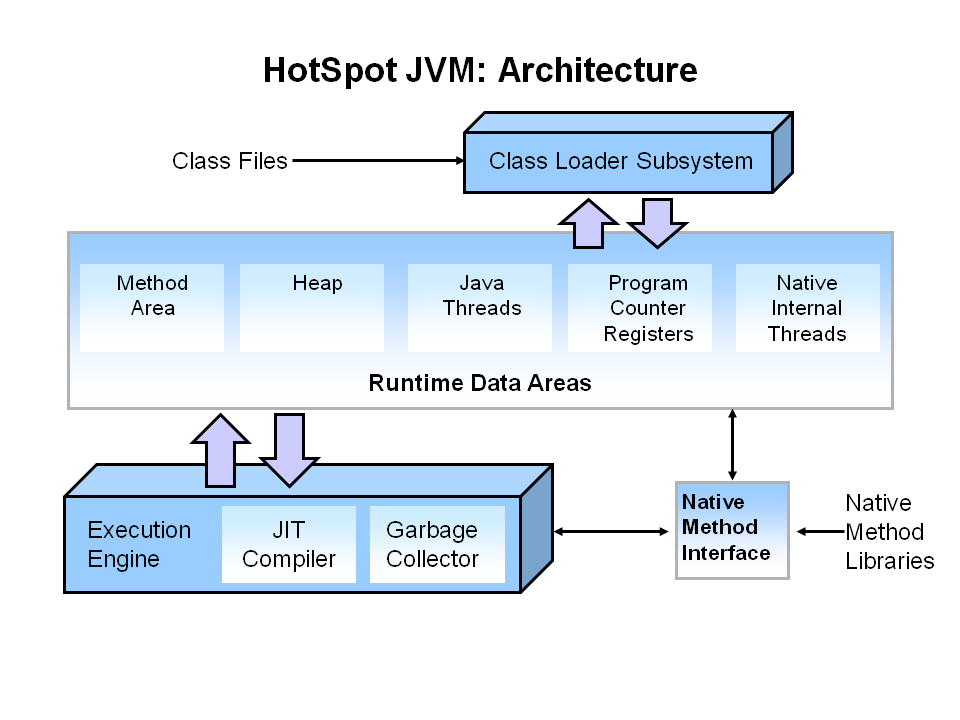
\includegraphics[width=0.95\textwidth, angle=0]{Meetings/February/02-24-22/2-24-22 1.PNG}
\caption{An illustration of the Java garbage collector's process.}
\label{fig:022422_1}
\end{figure}

\begin{figure}[htp]
\centering
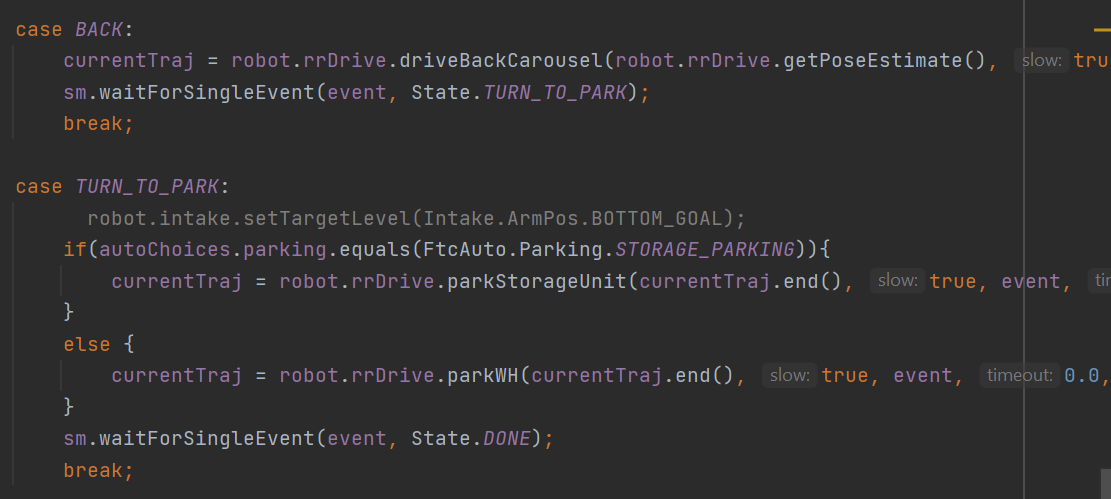
\includegraphics[width=0.95\textwidth, angle=0]{Meetings/February/02-24-22/2-24-22 2.PNG}
\caption{The two states where the code fails.}
\label{fig:022422_2}
\end{figure}


\whatsnext{
\begin{itemize}
    \item Continue refining autonomous programs before States. 
\end{itemize} 
}

